\documentclass[14pt,a4paper]{extarticle}

\usepackage[utf8]{inputenc}
\usepackage[T2A]{fontenc}
\usepackage{amssymb,amsmath,mathrsfs,amsthm}
\usepackage[russian]{babel}
\usepackage{graphicx}
\usepackage[footnotesize]{caption2}
\usepackage{indentfirst}
\usepackage{multicol}
\usepackage{listings}
\usepackage{float}
\usepackage{url}

\usepackage{enumitem}

%\usepackage[ruled,section]{algorithm}
%\usepackage[noend]{algorithmic}
%\usepackage[all]{xy}
\usepackage{booktabs}
\usepackage{graphicx}
\usepackage[table,xcdraw]{xcolor}
\usepackage{tcolorbox}

%Библиотека для блок-схем
\usepackage{tikz}
\usetikzlibrary{shapes,arrows}

% Параметры страницы
\textheight=24cm
\textwidth=16cm
\oddsidemargin=5mm
\evensidemargin=-5mm
\marginparwidth=36pt
\topmargin=-1cm
\footnotesep=3ex
%\flushbottom
\raggedbottom
\tolerance 3000
% подавить эффект "висячих стpок"
\clubpenalty=10000
\widowpenalty=10000
%\renewcommand{\baselinestretch}{1.1}
\renewcommand{\baselinestretch}{1.5} %для печати с большим интервалом

\newcommand{\angstrom}{\mbox{\normalfont\AA}}

\newtheorem{definition}{Определение} % задаём выводимое слово (для определений)
\newtheorem{example}{Замечание} % задаём выводимое слово (для определений)
\newtheorem{theorem}{Теорема} % задаём выводимое слово (для определений)
\newtheorem{construction}{Конструкция} % задаём выводимое слово (для определений)

\DeclareMathOperator*{\sgn}{sgn}
\DeclareMathOperator*{\var}{var}
\DeclareMathOperator*{\cov}{cov}
\DeclareMathOperator*{\law}{Law}

\newcommand{\1}{\mathbbm{1}}
\newcommand{\R}{\mathbb{R}}
\newcommand{\N}{\mathbb{N}}
\newcommand{\Z}{\mathbb{Z}}
\renewcommand{\P}{\mathbb{P}}
\newcommand{\E}{\mathbb{E}}

\newcommand{\independent}{\perp\!\!\!\!\perp}

\newcommand\cA{{\cal A}}
\newcommand\cE{{\cal E}}
\newcommand\cC{{\cal C}}
\newcommand\cF{{\cal F}}
\newcommand\cG{{\cal G}}
\newcommand\cK{{\cal K}}
\newcommand\cL{{\cal L}}
\newcommand\cB{{\cal B}}
\newcommand\cN{{\cal N}}
\newcommand\cM{{\cal M}}
\newcommand\cX{{\cal X}}
\newcommand\cD{{\cal D}}
\newcommand\cR{{\cal R}}
\newcommand\cP{{\cal P}}
\newcommand\cQ{{\cal Q}}
\newcommand\cS{{\cal S}}
\newcommand\cT{{\cal T}}
\newcommand\cV{{\cal V}}
\newcommand\cZ{{\cal Z}}

\newcommand{\textProposition}    {Предложение}
\newcommand{\textTask}    {Задача}

\begin{document}

\begin{center}

    {Всеволод Заостровский, 409 группа}\\
    {\bfseries Отчёт по задаче ''Итерационные методы решения систем линейных уравнений''.\\}
    \vspace{1cm}

\end{center}

\section{\textbf{Задача 1.}} Для решения системы линейных уравнений:
\begin{align*}
& -\frac{y_{k+1} - 2 y_k + y_{k-1}}{h^2} + p y_k = f_k, \;\;\;\;\; k = 1, \ldots, N - 1; \\
& y_0 = y_N = 0; \\
& h = \frac{1}{N}; \\
& p \geq 0.
\end{align*}
реализуйте метод Фурье (т.е. метод разложения по собственным векторам) для базисных функций:
\begin{equation}
    \psi_k^{(n)} = \sin(\frac{\pi n k}{N})
\end{equation}    

\textbf{Решение.} 
Сперва, найдём базисные функции:
$
\\
-y_{k+1} + 2 y_k - y_{k-1} + p y_k h^2 = f_k h^2 \\
y_{k+1} - 2(1 + \frac{p h^2}{2}) y_k + y_{k-1} = - f_k h^2 \\
$
Выпишем характеристическое уравнение и решим его однородный вариант:
$
\\
y_{k+1} - 2(1 + \frac{p h^2}{2}) y_k + y_{k-1} = 0. \\
y_{k+1} - 2 q y_k + y_{k-1} = 0 \\
\mu^2 - 2 q \mu + 1 = 0 \\
\mu_{1, 2} = q \pm \sqrt(q^2 - 1) \\
$
Пусть $\mu_1 = \mu_2$. Тогда:
$
\\
y_k = C_1 + k C_2 \\
y_0 = C_1 + 0 \cdot C_2 = 0 \rightarrow C_1 = 0 \\
y_N = 0 + N \cdot C_2 = 0 \rightarrow C_2 = 0 \\
$
Этот случай даёт тривиальное решение. Далее считаем, что $\mu_1 \neq \mu_2$.
$
\\
y_k = C_1 \mu_1^k + C_2 \mu^k_2 \\
y_0 = C_1 + C_2 = 0 \rightarrow C_1 = - C_2 \\
y_N = C_1 \mu_1^N + C_2 \mu_2^N \rightarrow C_1 (\mu_1^N - \mu_2^N) = 0  
\rightarrow (\text{случай $C_1 = 0$ тривиален}) \\
\rightarrow (\frac{\mu_1}{\mu_2}) ^ N = 1 
\rightarrow \frac{\mu_1}{\mu_2} = e^{\frac{2 \pi i k}{N}} \rightarrow \\
\text{из характеристического уравнения и теоремы Виета имеем $\mu_1 \mu_2 = 1$ } \\
\rightarrow \mu_1^2 = e^{\frac{2 \pi i k}{N}} \\
\rightarrow 
    \left\{
        \begin{array}{ccc}
        \mu_1 & = & e^{\frac{ \pi i k}{N}}, k \in \{1 \cdots N-1\} \\
        \mu_2 & = & e^{\frac{ - \pi i k}{N}}, k \in \{1 \cdots N-1\} \\
        \end{array}
    \right.
    \\
$
Отсюда получаем ответ\footnote{Ранее мы пренебрегли корнем $ - e^{\frac{ \pi i k}{N}}$, но он даёт тот же ответ, 
поскольку минус съедает константа.}:
$\\
y_k^{(n)} = C_1 (e^{\frac{ \pi i k}{N}} - e^{\frac{ - \pi i k}{N}}) = \hat C_1 \sin(\frac{\pi n k}{N}).
$



Вычислим $\lambda_n$ и заодно проверим, является ли найденная функция собственной: \\
$
{A \psi^{(n)}}_k =  -\frac{\psi^{(n)}_{k+1} - 2 \psi^{(n)}_k + \psi^{(n)}_{k-1}}{h^2} + p \psi^{(n)}_k \\
= -\frac{\sin(\frac{\pi n (k+1)}{N}) - 2 \sin(\frac{\pi n k}{N}) + \sin(\frac{\pi n (k-1)}{N})}{h^2} + p \sin(\frac{\pi n k}{N}) \\
= -\frac{\sin(\frac{\pi n k}{N}) \cos(\frac{\pi n}{N}) + \cos(\frac{\pi n k}{N}) \sin(\frac{\pi n}{N}) - 2 \sin(\frac{\pi n k}{N}) + \sin(\frac{\pi n k}{N}) \cos(\frac{\pi n}{N}) - \cos(\frac{\pi n k}{N}) \sin(\frac{\pi n}{N}) }{h^2} + p \sin(\frac{\pi n k}{N}) \\
= -\frac{\sin(\frac{\pi n k}{N}) \cos(\frac{\pi n}{N}) - 2 \sin(\frac{\pi n k}{N}) + \sin(\frac{\pi n k}{N}) \cos(\frac{\pi n}{N})}{h^2} + p \sin(\frac{\pi n k}{N}) \\
= -\frac{2 \sin(\frac{\pi n k}{N}) (\cos(\frac{\pi n}{N}) - 1)}{h^2} + p \sin(\frac{\pi n k}{N}) 
=  \sin(\frac{\pi n k}{N}) (-\frac{2 (\cos(\frac{\pi n}{N}) - 1)}{h^2} + p).
$ \\
Отсюда:
\begin{equation}
    \lambda_n = p - 2 N^2 (\cos(\frac{\pi n}{N}) - 1).
\end{equation}
Эти значения были проверены численно (см. /NumCheck). Кроме того, из указания к задаче:
\begin{equation}
    c_n = \frac{\left(f, \psi^{(n)} \right)}{\lambda_n \left(\psi^{(n)}, \psi^{(n)} \right)} 
            = \frac{2 \left(f, \psi^{(n)} \right)}{\lambda_n}.
\end{equation}
Решение же можно найти в виде:
\begin{equation}
    y_k = \sum_{n=1}^{N-1} c_n \psi_k^{(n)}.
\end{equation}
Огромные проблемы возникли всвязи с тем, что матрицей Фурье порядка $N$ прадлагается называть матрицу, 
размерность которой $N + 1$, при этом, подматрица из ненулевых элементов, для которой осмысленно
ставить задачу решения СЛУ имеет размерность $N - 1$. Об этом стоит помнить, во избежание изнурительной отладки. \par
Реализацию см. в файле ''solution.h'', незамысловатая система тестирования реализована в ''test1.c''.

\section{\textbf{Задача 2.}} Для решения системы линейных уравнений из \textbf{Задачи 1.} реализуйте метод Ричардсона.  
Проведите тестирование программы, сравнив теоретическую
и реальную скорость сходимости. Для этого на каждом $k$-ом шаге, $k = 0,1, \ldots $ итерационного
процесса сохраните в некоторый файл очередную тройку.

\textbf{Решение.} 
Реализацию см. в файле ''solution.h'', незамысловатая система тестирования реализована в ''test2.c''. \par
Фактически реализован функционал (правда, не самый эффективный), позволяющий применить метод к любой матрице.
Очень остро здесь стоит вопрос определения $m$ и $M$ (см. файл ''../LinAlg.pdf''). Для матрицы из задачи 1 
есть явная формула собственных значений, благодаря чему удалось добиться хорошего приближения к теоретической сходимости. 
Однако, если бы не было известной формы, то найти их с приемлемой точностью представлялось бы задачей, вычислительная сложность которой
сравнима со сложностью решения всей системы. При этом, неправильное $\tau$, как показали многочисленные отладочные тесты,
не включенные в отчет, может очень сильно испортить сходимость. \par
По результатам тестирования был построен график (для вывода ./LS2 50 1000 100 out.txt, те матрица порядка 50, до 1000 итераций 
с $p = 100$). См. рисунок.

\begin{figure}
    \centering
    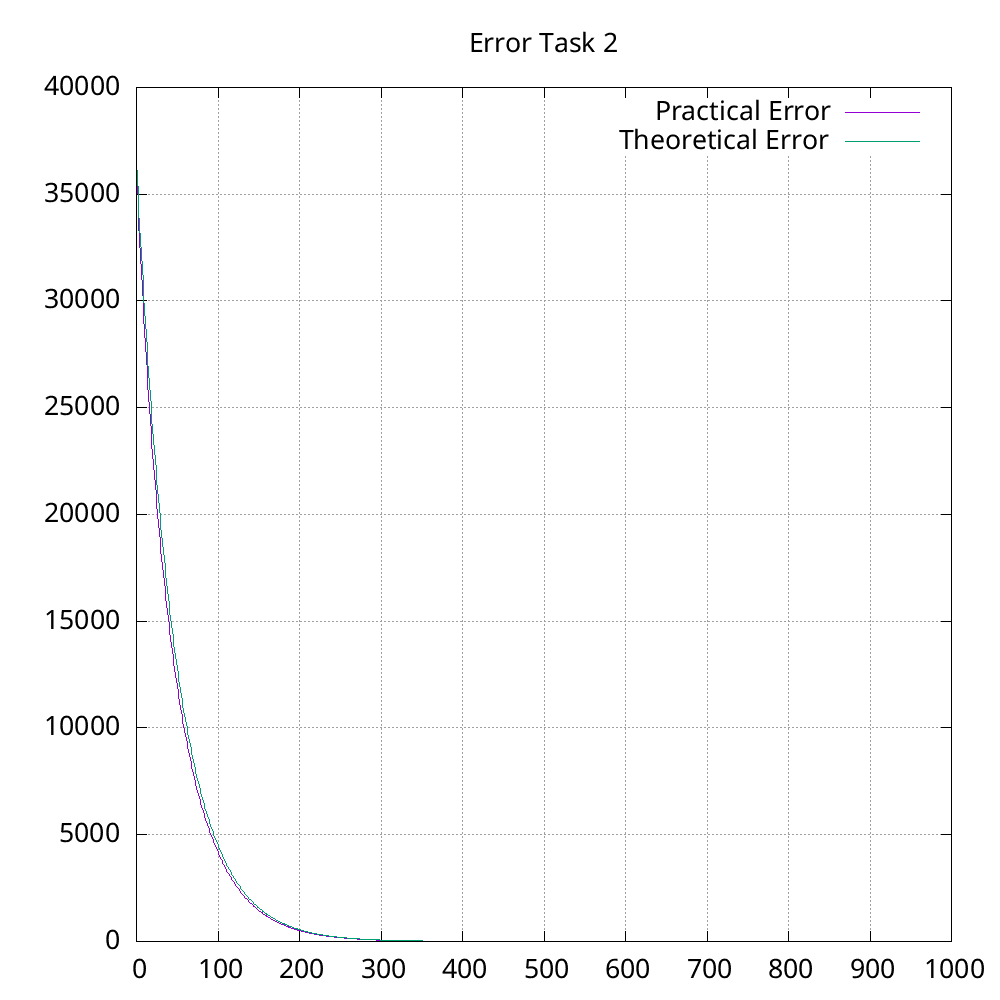
\includegraphics[scale=0.55]{Error2.png}
    \caption{Ошибка метода Ричардсона решения СЛУ, определяемого матрицей типа Фурье (задача 1).}
\end{figure}


\section{\textbf{Задача 3.}} Для решения системы линейных уравнений:
\begin{align*}
& -\frac{y_{k+1} - 2 y_k + y_{k-1}}{h^2} + p_k y_k = f_k, \;\;\;\;\; k = 1, \ldots, N - 1; \\
& y_0 = y_N = 0; \\
& h = \frac{\pi}{N}; \\
& p_k = 1 + \sin^2(\pi k h).
\end{align*}
реализуйте метод с предобуславливателем.

\textbf{Решение.} 
Реализацию см. в файле ''solution.h'', незамысловатая система тестирования реализована в ''test3.c''. \par
Фактически, приведенная реализация поддерживает любой предобуславливатель. В том числе, как требовалось в задаче, 
реализовано обращение матрицы методом Фурье. \par
По результатам тестирования был построен график (для вывода ./LS3 50 1000 100 out.txt, те матрица порядка 50, до 1000 итераций 
с $p = 100$). См. рисунок.

\begin{figure}
    \centering
    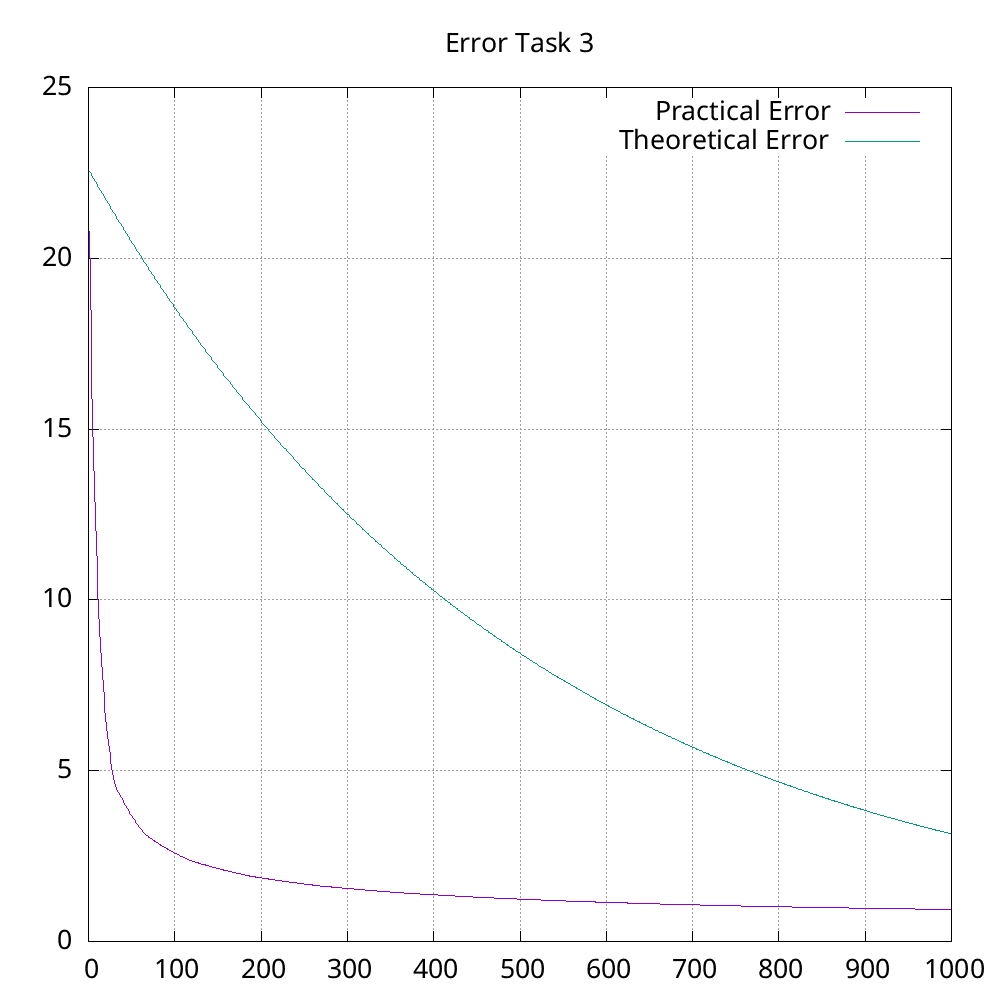
\includegraphics[scale=0.55]{Error3.png}
    \caption{Ошибка метода решения СЛУ, определяемого матрицей типа Фурье (задача 3), с предобуславливателем.}
\end{figure}

\end{document}